\documentclass{standalone}
\usepackage{tikz}

\usetikzlibrary{shapes.geometric, arrows}

\begin{document}

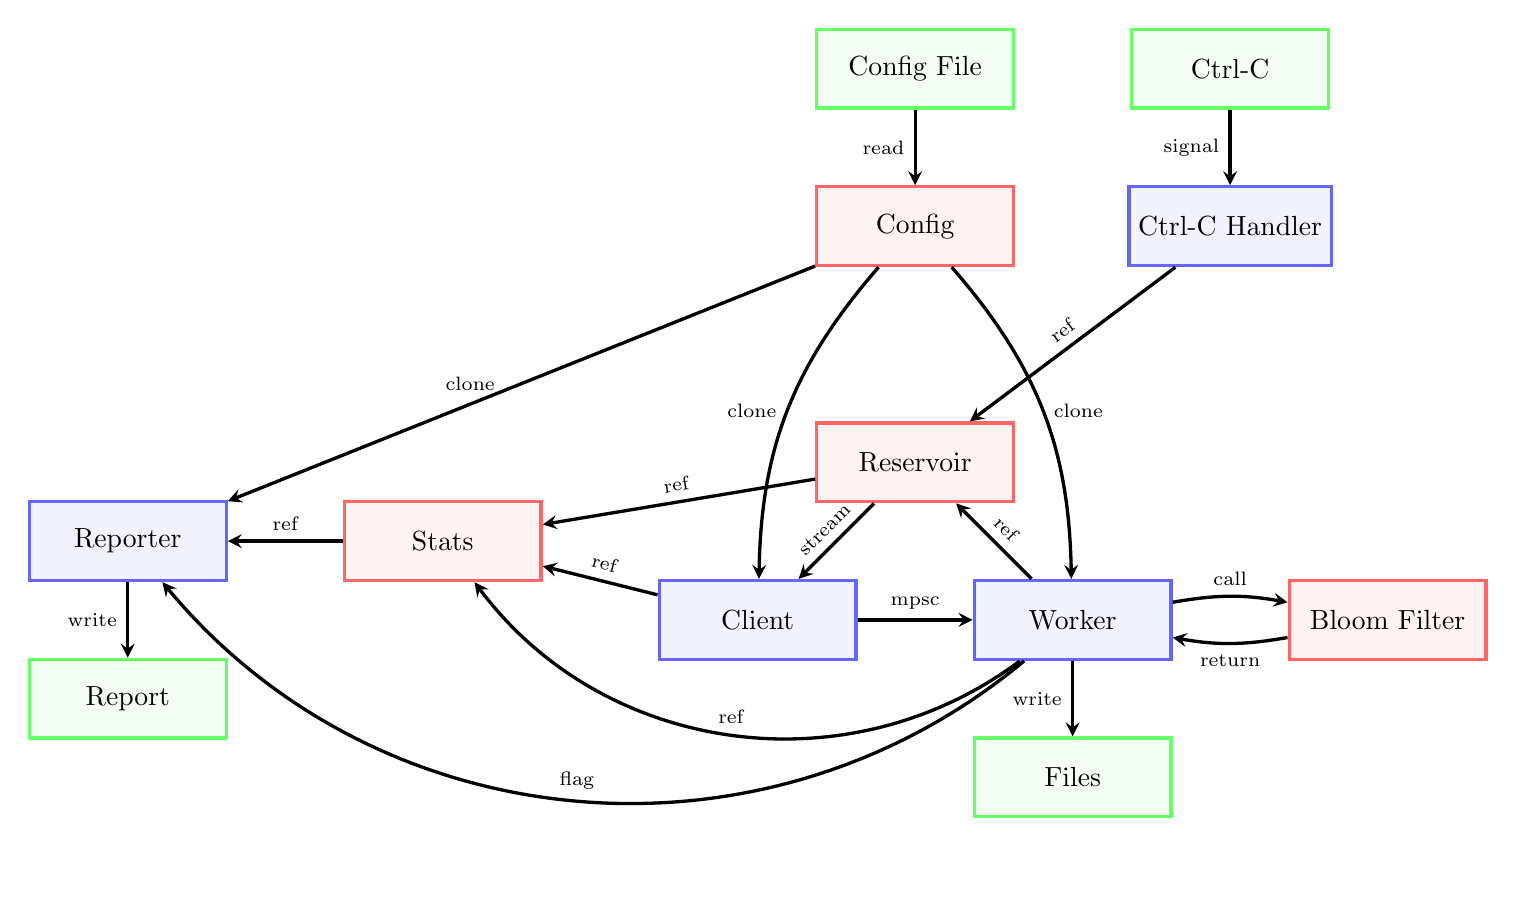
\begin{tikzpicture}[node distance=1.75cm]
\tikzstyle{entity_struct}=[rectangle, draw=red!60, fill=red!5, very thick, minimum width=2.5cm, minimum height=1cm];
\tikzstyle{entity_thread}=[rectangle, draw=blue!60, fill=blue!5, very thick, minimum width=2.5cm, minimum height=1cm];
\tikzstyle{entity_outside}=[rectangle, draw=green!60, fill=green!5, very thick, minimum width=2.5cm, minimum height=1cm];
\tikzstyle{empty}=[];
\tikzstyle{arrow} = [->, >=stealth, very thick]

\node [entity_outside] at (4,5) (Ctrl-C) {Ctrl-C};
\node [entity_thread] at (4,3) (Ctrl-C Handler) {Ctrl-C Handler};
\node [entity_outside] at (0,5) (Config File) {Config File};
\node [entity_struct] at (0,3) (Config) {Config};
\node [entity_struct] at (0,0) (Reservoir) {Reservoir};
\node [entity_thread] at (-2,-2) (Client) {Client};
\node [entity_thread] at (2,-2) (Worker) {Worker};
\node [entity_struct] at (-6,-1) (Stats) {Stats};
\node [entity_thread] at (-10,-1) (Reporter) {Reporter};
\node [entity_outside] at (-10,-3) (Report) {Report};
\node [entity_outside] at (2,-4) (Files) {Files};
\node [entity_struct] at (6,-2) (Bloom Filter) {Bloom Filter};


\draw[arrow] (Reservoir) -- node[sloped, anchor=center, above] {\scriptsize{stream}} (Client);
\draw[arrow] (Client) -- node[sloped, anchor=center, above] {\scriptsize{mpsc}} (Worker);
\draw[arrow] (Worker) -- node[sloped, anchor=center, above] {\scriptsize{ref}} (Reservoir);

\draw[arrow] (Worker) -- node[anchor=center, left] {\scriptsize{write}} (Files);
\draw[arrow] (Reporter) -- node[anchor=center, left] {\scriptsize{write}} (Report);
\draw[arrow] (Stats) -- node[anchor=center, above] {\scriptsize{ref}} (Reporter);
\draw[arrow] (Config File) -- node[anchor=center, left] {\scriptsize{read}} (Config);
\draw[arrow] (Ctrl-C) -- node[anchor=center, left] {\scriptsize{signal}} (Ctrl-C Handler);
\draw[arrow] (Ctrl-C Handler) -- node[sloped, anchor=center, above] {\scriptsize{ref}} (Reservoir);

\draw[arrow] (Worker) to [bend left=10] node[anchor=center, above] {\scriptsize{call}} (Bloom Filter);
\draw[arrow] (Bloom Filter) to [bend left=10] node[anchor=center, below] {\scriptsize{return}} (Worker);

\draw[arrow] (Reservoir) -- node[sloped, anchor=center, above] {\scriptsize{ref}} (Stats);
\draw[arrow] (Client) -- node[sloped, anchor=center, above] {\scriptsize{ref}} (Stats);
\draw[arrow] (Worker) to [bend left=45] node[anchor=center, above] {\scriptsize{ref}} (Stats);
\draw[arrow] (Worker) to [bend left=45] node[anchor=center, above] {\scriptsize{flag}} (Reporter);


\draw[arrow] (Config) to [bend left=20] node[anchor=center, right] {\scriptsize{clone}} (Worker);
\draw[arrow] (Config) to [bend right=20] node[anchor=center, left] {\scriptsize{clone}} (Client);
\draw[arrow] (Config) -- node[anchor=center, left, xshift=-.2cm] {\scriptsize{clone}} (Reporter);


\end{tikzpicture}
\end{document}